\documentclass[12pt]{article}
%	options include 12pt or 11pt or 10pt
%	classes include article, report, book, letter, thesis

\usepackage{amsmath}
\usepackage{graphicx}
%\usepackage{graphics}
%\usepackage{subfigure}
\usepackage{bm}
\usepackage{subfig}
\usepackage{float}

\usepackage{listings}
\usepackage[usenames, dvipsnames]{color}
\usepackage{xcolor}

\lstset { %
    language=C++,
    backgroundcolor=\color{black!5}, % set backgroundcolor
    basicstyle=\footnotesize,% basic font setting
}

\title{Characteristics of advection-diffusion equation}
%对流扩散方程
\author{Fangbo Wang \\   }
\date{September 2017}

\begin{document}
\maketitle

The advection-diffusion equation is a well-known PDE which can capture advection and diffusion effects that are popular in the physical world. It can be used in fluid mechanics (Navier-Stokes equation), stochastic differential theory (Fokker-Planck equation), finance modeling (Black-Scholes equation), etc. The equation can be written as below:
\begin{equation}
\frac{\partial f}{\partial t}=N_1 \frac{\partial f}{\partial x} + N_2 \frac{\partial^2 f}{\partial x^2}
\end{equation}
Where $N_1$ and $N_2$ are the advection and diffusion coefficients, respectively.

There are some interesting characteristics for advection-diffusion equation which we will explore below in an probabilistic context. Assume we have an initial condition of a standard normal probability density function. The boundary is set to be [-20 20] for numerical computation which is actually infinite, and also an reflecting boundary is employed \cite{sett}. 

Assume $timestart=0, dt=0.01, N_1=100, N_2=1$ as the standard parameters. 

First of all, we can change the advection coeffcient to see its effect. As can be seen in Fig. \ref{fig1}, positive $N_1$ would shift to right and negative $N_1$ would shift to left. The advection coeffecient can be understood as the moving velocity of a particle. The moving distance is 5 with velocity 500 and time 0.01 second as can be seen on the bottom right plot.


\begin{figure}[!htbp]
\begin{center}

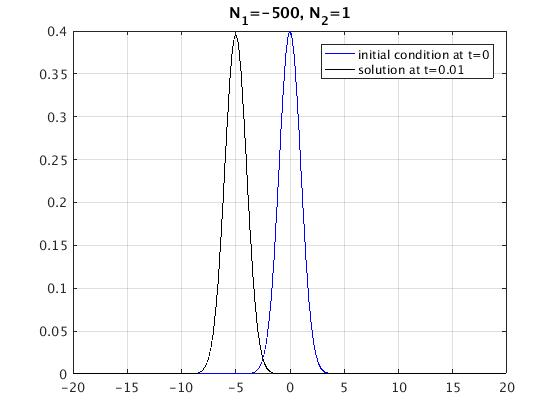
\includegraphics[width=0.46\textwidth]{advec-500.jpg} 
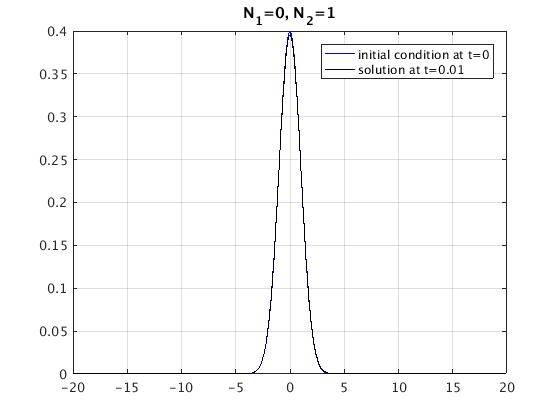
\includegraphics[width=0.46\textwidth]{advec0.jpg}  \\
\hspace*{0.2truecm}
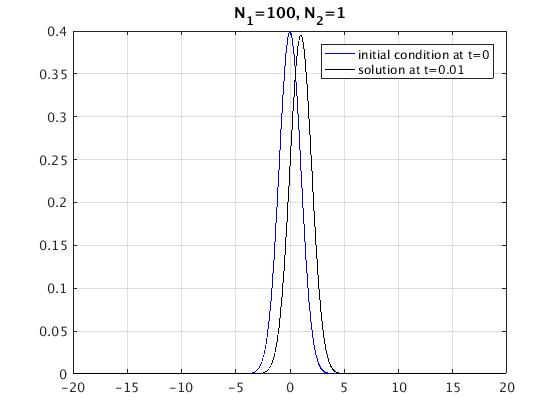
\includegraphics[width=0.46\textwidth]{norm.jpg}  
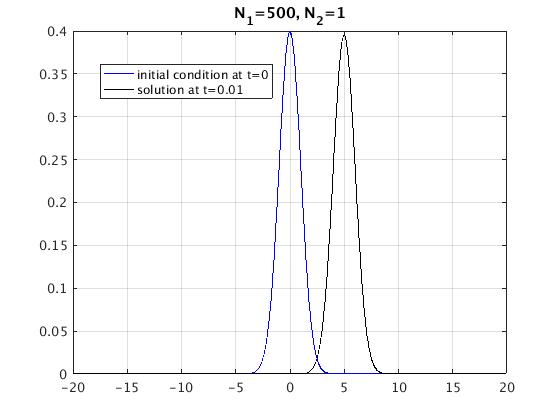
\includegraphics[width=0.46\textwidth]{advec500.jpg}  \\

\caption{Effects of changing advection coefficient.} 
\label{fig1}
\end{center}
\end{figure}

Similarly, the effect of diffusion coefficient can be shown in Fig. \ref{fig2}. 
With positive diffusion coefficient, the shape of the function would diffuse to have a larger spreadness. However, negative diffusion coefficient which indicating concentration would render the equation ill-posed and difficult to solve the problem. It can be categorized as a backward heat equation. It's common to see high frequency oscillations in the solution, that's because the negative diffusion process behaves like differention to make the solution coarser than initial condition. However, positive diffusion process behaves like integration to make the solution smoother than initial condition \cite{Threfethen}. Numerous techniques have been proposed to overcome this ill-posed problem, and regularization is one of them, see ref \cite{Fu}. 

Furthermore, negative diffusion coefficient is an inverse process which might have multiple possible solutions. Only equation with very small negative diffusion coefficient would be solved. Regarding this specific problem, the smallest possible value of $N_2$ is -0.2. Solution with negative diffusion coefficient would have smaller standard deviation due to concentration effect (standard deviation=0.998). 

\begin{figure}[H]
\begin{center}

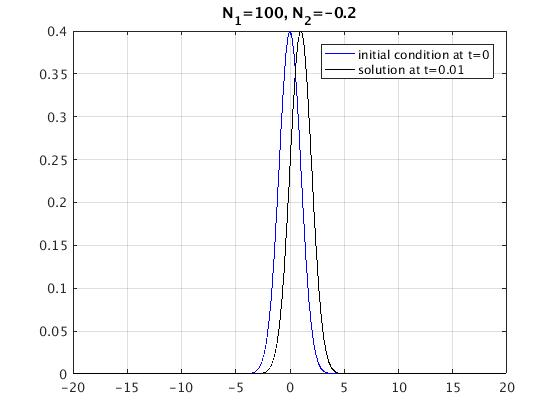
\includegraphics[width=0.46\textwidth]{diffu-02.jpg} 
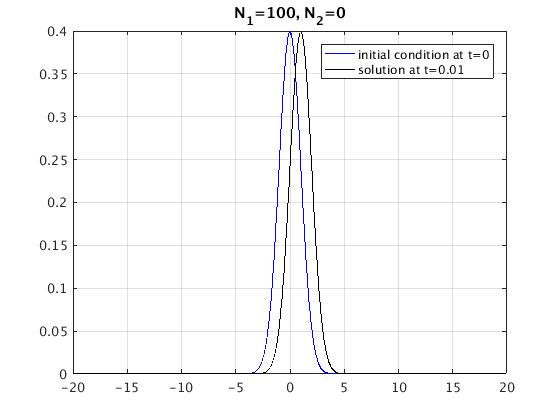
\includegraphics[width=0.46\textwidth]{diffu0.jpg}  \\
\hspace*{0.2truecm}
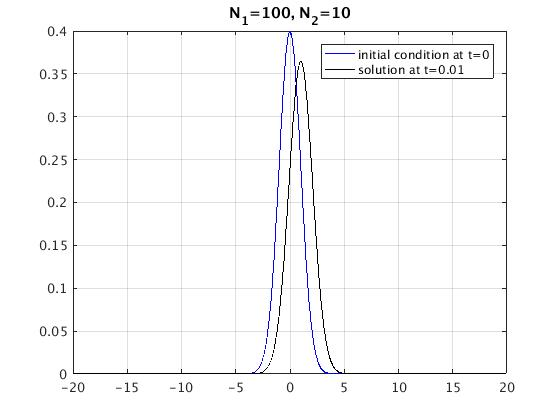
\includegraphics[width=0.46\textwidth]{diffu10.jpg}  
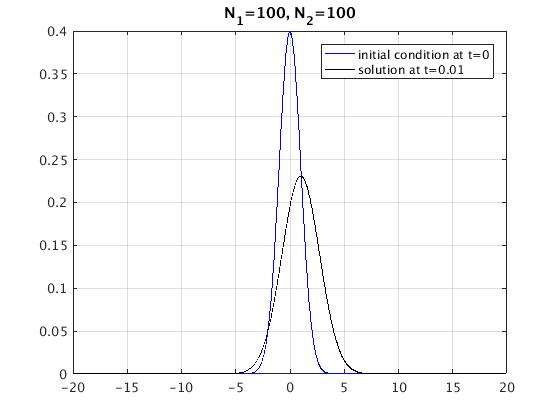
\includegraphics[width=0.46\textwidth]{diffu100.jpg}  \\

\caption{Effects of changing diffusion coefficient.} 
\label{fig2}
\end{center}
\end{figure}

Furthermore, the effect of changing starting time is shown in Fig. \ref{fig3}. It is observed that starting time doesn't have influence on the result.

\begin{figure}[H]
\begin{center}

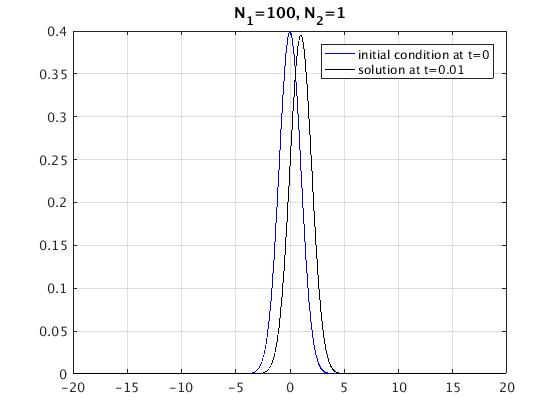
\includegraphics[width=0.46\textwidth]{norm.jpg} 
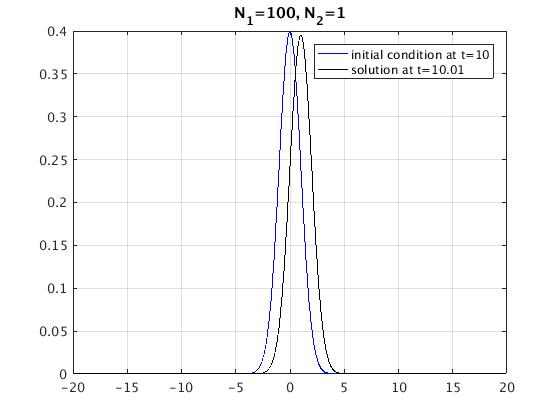
\includegraphics[width=0.46\textwidth]{t10.jpg}  \\
\hspace*{0.2truecm}

\caption{Effects of changing starting time.} 
\label{fig3}
\end{center}
\end{figure}

The effect of changing the incremental time is shown in Fig. \ref{fig4}. It is seen that longer incremental time would both advect and diffuse the function along time. 

\begin{figure}[H]
\begin{center}

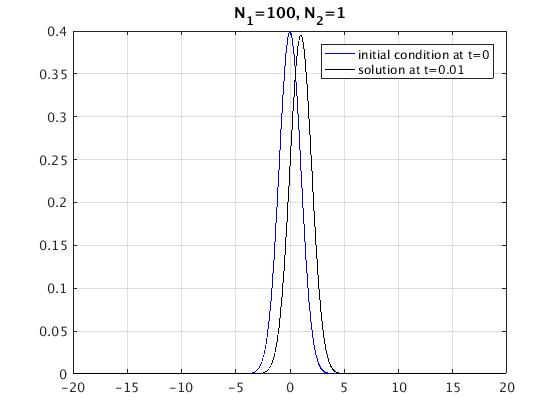
\includegraphics[width=0.46\textwidth]{norm.jpg} 
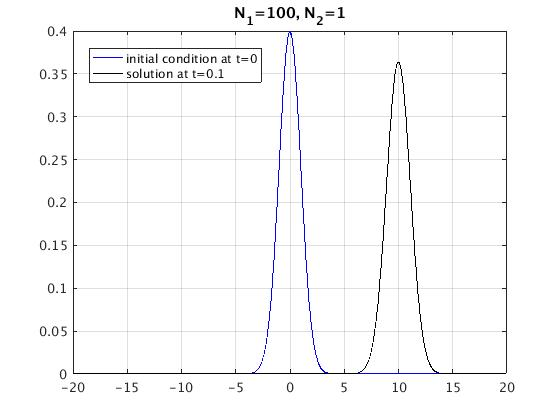
\includegraphics[width=0.46\textwidth]{dt01.jpg}  \\
\hspace*{0.2truecm}

\caption{Effects of changing incremental time.} 
\label{fig4}
\end{center}
\end{figure}


Below is the main.m script file.
\begin{lstlisting}
clc; clear;
leftbound=-20; rightbound=20; meshpoint=2000;
stressmesh=linspace(leftbound, rightbound, meshpoint);
% standard normal assumption;
u00=exp(-stressmesh.*stressmesh/2)/sqrt(2*pi); 
timestart=10; dt=0.01;
N1=100;  N2=1;        

[sol]=solve_FPK(u00, N1, N2, timestart, dt, leftbound, rightbound, meshpoint);

 plot(stressmesh, u00, 'b'); hold on;
 plot(stressmesh, sol, 'k'); grid on;
 legend('initial condition at t=0', 'solution at t=0.01' )
 title('N_1=100, N_2=1')

\end{lstlisting}

\vspace{1cm}
Below is the solve\_FPK function file

\begin{lstlisting}

function [sol]=solve_FPK(u00, N1, N2, timestart, timeincrement_small, leftbound,
 		rightbound, meshpoint)

    x = linspace(leftbound, rightbound, meshpoint);
    t = linspace(timestart,  timestart+timeincrement_small , 101);
    m = 0;
    solution = pdepe(m,@pdex1pde,@pdex1ic,@pdex1bc,x,t);
    sol=solution(end,:);

    function [c,f,s] = pdex1pde(x,t,u,DuDx)
        c = 1;
        f = N2*DuDx;
        s = -N1*DuDx;
    end

    function u0 = pdex1ic(x)
        u0=interp1(  linspace(leftbound, rightbound, meshpoint), u00, x );
    end

    function [pl,ql,pr,qr] = pdex1bc(xl,ul,xr,ur,t)
        pl = N1*ul;
        ql = -1;
        pr = N1*ur;
        qr = -1;
    end

end


\end{lstlisting}

\begin{thebibliography}{9}
\bibitem{sett} 
Arezoo Sadrinezhad, Kallol Sett and S. I. Hariharan. 
Efficient solution algorithms for multiaxial probablistic elasto-plastic constitutive simulations of soils.
\textit{Int J Numer Anal Mech Geomech}. 
2017; 0:1-21.
 
\bibitem{Fu} 
Chuli Fu, Xiangtuan Xiong and Zhi Qian. 
Fourier regularization for a backward heat equation.
\textit{Jounal of Mathematical Analysis and Applications}. 
2007; 331:471-480.

\bibitem{Threfethen} 
Lloyd N. Trefethen and Kristine Embree. 
The PDE Coffee Table Book. Chapter 3. Backward heat equation...ill-posed problems and regularisation.
\textit{https://people.maths.ox.ac.uk/trefethen/pdectb.html}. 
2011.

\end{thebibliography}


\end{document}
